\chapter{Teorema de la dimensión}

\noindent En los dos capítulos anteriores, hemos definido la dimensión de un módulo en un contexto global (proyectivo, graduado) y en un contexto local (filtrado). La ventaja técnica de estas definiciones es que están basadas en el polinomio de Hilbert. Esto nos permite estudiar módulos complicados relacionándolos con otros módulos más simples mediante sucesiones exactas.

Sin embargo, desde un punto de vista geométrico, el concepto de dimensión de un módulo no es muy convincente, ya que es a todas luces un despropósito llamar ``dimensión'' a una propiedad puramente algebraica de un objeto puramente algebraico. Para superar esta dificultad, daremos una interpretacion geométrica intuitiva para los módulos que nos interesan.

Sea $R$ el anillo de coordenadas de una variedad afín $Y \subset \A^n$. Los $R$-módulos no triviales más sencillos son de la forma $R/\p$, donde $\p \subset R$ es un ideal primo. Visualmente, $R/\p$ es una muralla construida sobre $V(\p)$. El resto de $Y$ es terreno vacío sin construir. En particular, si $\m \subset R$ es el ideal maximal de un punto $p \in V$, decimos que $R/\m$ es un \textit{haz rascacielo} sobre $p$.

Más generalmente, sea $M$ un $R$-módulo finitamente generado y sean $\p_1 \dots \p_r \subset R$ los ideales primos que aparecen en las filtraciones limpias de $M$. Visualmente, $M$ es la superposición\footnote{En el sentido del ``principio de superposición'' del álgebra lineal.} de las murallas $R/\p_i$. Esta clase de objetos se conocen como \textit{haces coherentes} sobre la variedad $Y$.

Para cada ideal primo $\p \subset R$, el \textit{tallo} $M_\p$ describe el comportamiento de $M$ en una vecindad genérica de $V(\p)$. Los \textit{fibrados vectoriales} corresponden de manera natural a los haces coherentes tales que cada tallo $M_\p$ es un $R_\p$-módulo libre. (Ver \cite[p. 291]{gortz}.)

\begin{definition}
El \textit{soporte} de $M$, denotado $S(M)$, es el conjunto algebraico conformado por todos los puntos $p \in Y$ tales que el tallo $M_\m$ sobre el ideal maximal $\m = I(p)$ es no trivial.
\end{definition}

De manera análoga al caso afín, si $R$ es el anillo de coordenadas homogéneo de una variedad proyectiva $Y \subset \P^n$, los $R$-módulos graduados finitamente generados se pueden interpretar como haces coherentes sobre $Y$. En este caso...

\begin{definition}
El \textit{soporte} de $M$, denotado $S(M)$, es el conjunto algebraico conformado por todos los puntos $p \in Y$ tales que el tallo $M_\p$ sobre el ideal primo homogéneo $\p = I(p)$ es no trivial.
\end{definition}

En este capítulo, demostraremos que la dimensión de $M$ definida algebraicamente no es otra cosa que la dimensión de su soporte definida geométricamente.

\begin{figure}[h]
    \centering
    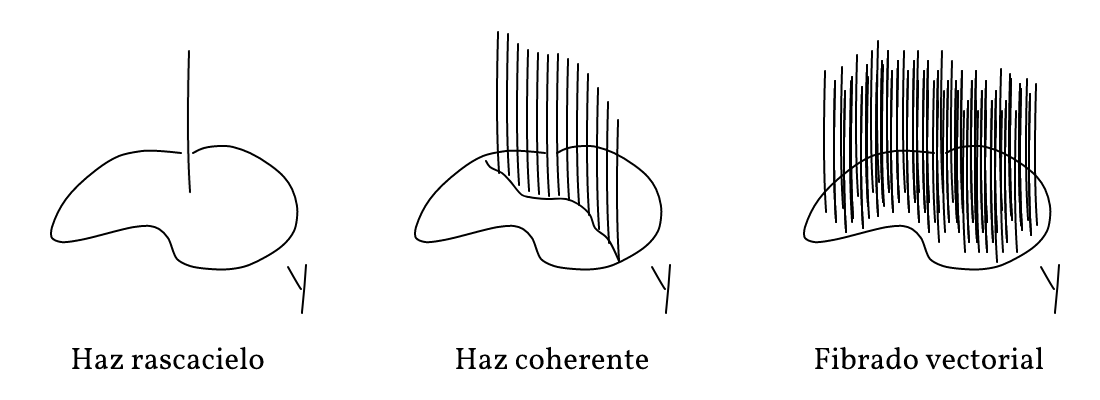
\includegraphics[scale=0.3]{ch5/sheaf.png}
    \caption{Ejemplos de haces}
\end{figure}
